%%%%%%%%%%%%%%%%%%%%%%%%%%%%%%%%%%%%%%%%%%%%%%%%%%%%%%%%%%%%%%%%%%%%%%%%
% Preamble
%%%%%%%%%%%%%%%%%%%%%%%%%%%%%%%%%%%%%%%%%%%%%%%%%%%%%%%%%%%%%%%%%%%%%%%%
\documentclass[11pt]{article}
%
% Packages and other includes
% Pagination
\usepackage[letterpaper, margin=1in]{geometry}
\usepackage{emptypage}
%
% Fonts
\usepackage[T1]{fontenc} % best for Western European languages
\usepackage{lmodern} % Latin Modern instead of CM
\usepackage{textcomp} % required to get special symbols
%
% Math
\usepackage{amsmath, amssymb}
\usepackage{braket}
%
% Graphics, floats, tables
\usepackage{graphicx, color, float, array}
%
% Hyperlinks
\usepackage{hyperref}
%
%
% Definitions and settings
% Paragraph indent and spacing
\setlength{\parskip}{0.4\baselineskip}
\setlength{\parindent}{0in}
%
%
% Title, authors, date
\title{\textbf{Worksheet 3}}
\date{\vspace{-2em}January 18, 2022}
%
%
%%%%%%%%%%%%%%%%%%%%%%%%%%%%%%%%%%%%%%%%%%%%%%%%%%%%%%%%%%%%%%%%%%%%%%%%
% Main document
%%%%%%%%%%%%%%%%%%%%%%%%%%%%%%%%%%%%%%%%%%%%%%%%%%%%%%%%%%%%%%%%%%%%%%%%
%

\begin{document}

\maketitle

Weekly homework assignments are posted approximately one week prior to the
due date. Collaborations are encouraged and students must report all collaborators
in writing on each assignment. All external sources (websites, books) must be
properly cited. Additional problems are listed at the end of each assignment.
This week's assignment is due \textit{Tuesday, Jan 25th at 10:00am.}


\textbf{Real Gases}

1. (2 pts) The pressure of a sample of hydrogen fluoride is lower than expected and, as the
temperature is increased, rises more quickly than the ideal gas law predicts.
Suggest an explanation in words and/or illustrations.

\vspace{1in}

\textbf{First Law of Thermodynamics}

2. (2 pts) Below there are pictures showing a molecular view of a system
undergoing a change. In each case, predict the signs of $q$ and $w$ for
 each process. Explain what is happening to the system.

\begin{center}
  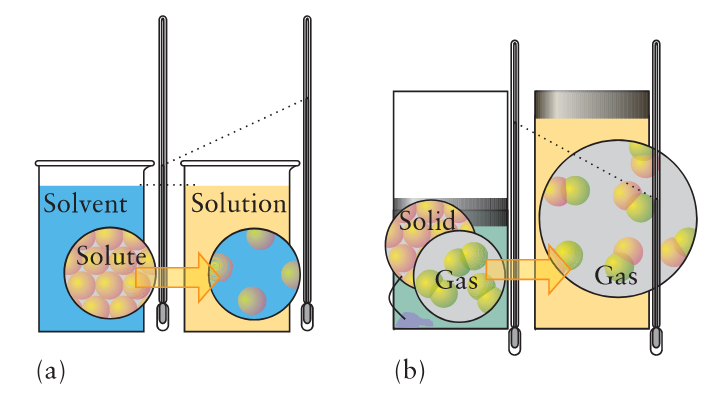
\includegraphics[scale=0.35]{phase_change.png}
\end{center}

\vspace{1.5in}

\textbf{Enthalpy $\Delta H$}

3. (4 pts) Carbon disulfide can be prepared from coke (an impure form of carbon) and
elemental sulfur

\begin{center}
  4 C(s) + S$_8$(s) $\rightarrow$ 4 CS$_2$(l) \, $\Delta H_r = +358.8\text{kJ}$.
\end{center}

(a) How much heat is absorbed in the reaction of $1.25\text{mol}$ S$_8$?

(b) Calculate the heat absorbed in the reaction of $197\text{g}$ of carbon
with an excess of sulfur.

(c) If the heat absorbed in the reaction was $415\text{kJ}$, how much of CS$_2$
was produced?

\vspace{2in}

4. (4 pts) Calculate the heat generated by a reaction mixture of $13.4\text{L}$ of SO$_2$
at $1.00\text{atm}$ and $273\text{K}$ and $15.0\text{g}$ of oxygen in the reaction

\begin{center}
  2 SO$_2$(g) + O$_2$(g) $\rightarrow$ 2 SO$_3$(g) \, $\Delta H_r = -198\text{kJ}$.
\end{center}

\vspace{1in}

5. (4 pts) An experimental automobile burns hydrogen for fuel. At the beginning of a test
drive, the rigid 30.0-L tank was filled with hydrogen at 16.0atm and 298K. At the end of
the drive, the temperature of the tank was still 298K, but its pressure was 4.0atm.

(a) How many moles of H$_2$ were burned during the drive?

(b) How much heat, in kilojoules, was given off by the combustion of that amount of
hydrogen?


%6. (4 pts) \textbf{Rankine Cycle}. The Rankine Cycle or Rankine Vapor Cycle is a
%widely used process by power plants such as caol-fired power plants and nuclear
%reactors. This thermodynamic cycle converts heat into mechanical energy which
%gets transformed into electricity. What
%
%(a)
%
%(b)
%
%\begin{center}
%  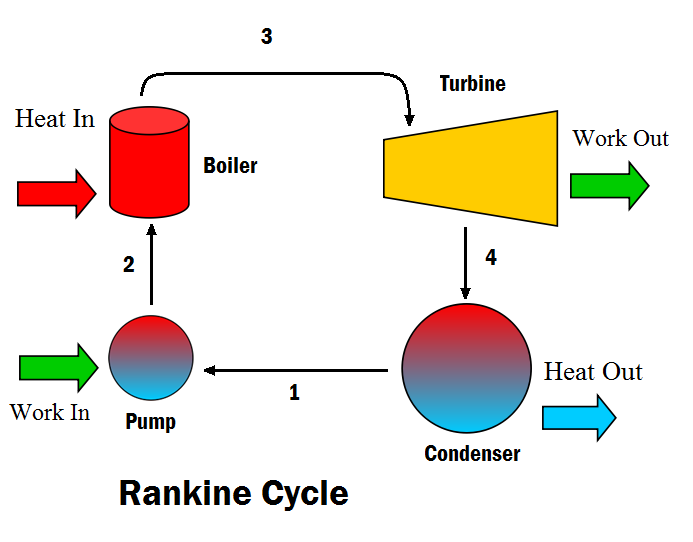
\includegraphics[scale=0.5]{rankine_cycle.png}
%\end{center}
%
% Rankine Cycle
%
% https://energyeducation.ca/encyclopedia/Rankine_cycle
%
% https://www.youtube.com/watch?v=hEzBdzPjf6I

\end{document}
